This section serves as an introduction of \Gls{TN} manipulations. The overview mainly focusses on \Gls{MPS}/\Gls{MPO} networks, but most of the operations translate to the 2D case.
The \Glspl{MPS} are processed by transforming the tensor into a matrix, performing some matrix calculations and casting it back into its original form. In this way, the standard methods from linear algebra can be used. This section gives some examples how this is done in practice.

\subsection{Basics}

\subsubsection{Grouping legs}
One of the most basic manipulations is to group some legs of a tensor into one leg:
\begin{equation}
    \begin{split}
        T^{i_1 i_2 j_1 j_2} &=  \expH{2}{$T$}{{"$i_1$","$i_2$"}}{{"$j_1$","$j_1$"}}{} \\
        & \cong \expH{2}{$T$}{{"-","-"}}{{"-","-"}}{{"$(i_1 j_1 )$","$(i_2 j_2)$"}} \\
        &= T^{ (i_1 j_1 ) (i_2 j_2) } \\
    \end{split}
\end{equation}
The dimension of the new leg is the product of the dimension of the individual legs. Contracting legs separately or in merged form gives the same result. The 4 leg tensor and matrix contain exactly the same information. Manipulating this in memory requires both permute and reshape commands. This requires some time as the internal representation of the matrix changes.

\subsubsection{Virtual levels}
A matrix can be split in smaller block matrices. Similarly, a leg of a tensor can be split in virtual levels. Each virtual level has its own dimension. Contracting a common leg means summing over all the virtual levels, and performing a normal contraction for each virtual level. These virtual level will be useful in \cref{chap4}.

\subsubsection{Decomposition} \label{decompMPO}
\def \figone {\expH{2}{$O^{u v,v w}$}{{"$i_1$","$i_2$"}}{{"$j_1$","$j_1$"}}{{"u","w"}}}

The grouping above can be applied to decompose a tensor into 2 tensors with matrix techniques. An example is
\begin{equation}
    \begin{split}
        \figone &= O^{i_1 i_2 j_1 j_2 }_{\alpha_u \gamma_w} \\
        &\cong O^{u w}_{ (\alpha_u i_1 j_1) (\gamma_w i_2 j_2) } \\
        &= O^{u v}_{(\alpha_u i_1 j_1) \alpha_v } O^{v w}_{ \alpha_v (\alpha_w i_2 j_2) } \\
        &\cong \mpo{2}{{"u","v","w"}}{{"$i_1$","$i_2$"}}{{"$j_1$","$j_1$"}}{}{}.
    \end{split}
\end{equation}
The indices U, V and W represent virtual levels. Step 2 reshapes and groups the indices into one index on the left and one on the right. The dimension of this index is the product of the separate dimensions. Step 3 decomposes the matrix into a product of 2 matrices. The last step transforms the indices back to separate legs. The rank of the original matrix is kept the same if
\begin{equation}
    \dim{v} = \min( \dim{u}, \dim{w}) \cdot d ^2 .
\end{equation}
Here, d is the physical dimension. Many different matrix decompositions exist. Some useful examples here are \Gls{SVD} decomposition, eigenvalue decomposition, QR, $\cdots$.

\subsubsection{Truncation}

The above procedure also gives a way to truncate the bond dimension: first take together 2 neighbouring sites, then perform an \Gls{SVD} Decomposition: $T = U \Sigma V^{\dagger}$. Split as
\begin{equation}
    T = \begin{bmatrix}
        U_1 & U_2 \\
    \end{bmatrix} \begin{bmatrix}
        \Sigma_1 & 0        \\
        0        & \Sigma_2 \\
    \end{bmatrix} \begin{bmatrix}
        V_1 & V_2\\\end{bmatrix}^{\dagger},
\end{equation}
where $\Sigma_1$ contains the n largest singular values. Then $\hat{T} = U_1 \Sigma_1 V_1^{\dagger}$ is the best rank n approximation to the original tensor.
\begin{equation}
    min_{rank(A) \leq n } \| T-A  \|  = \| T- \hat{T}  \|
\end{equation}

\subsubsection{Inversion}

\def \figone {\expH{2}{$A$}{{"$i_1$","$i_2$"}}{{"$j_1$","$j_2$"}}{{"u",}}}
\def \figthree {\expH{3}{$B$}{{"$i_1$","$i_2$","$i_3$"}}{{"$j_1$","$j_2$","$j_3$"}}{{"u","v"}}}
\def \figtwo {\mpo{1}{{,"v"}}{{"$i_3$",}}{{"$j_3$",}}{}{}}

Suppose we want to find a \Gls{MPO} O for given tensors A and B such that the following holds
\begin{equation}
    \combineTikz{ \figone }{\figtwo}{1.8} =  \figthree .
\end{equation}
The indices can be taken together in the following way: $\alpha = (u i_1 j_1  i_2 j_2)$ and $\beta = (i_3 j_3 v)$. The problem is now rewritten as
\begin{equation}
    A_{\alpha \gamma} O_{\gamma \beta} = B_{\alpha \beta} .
\end{equation}
This is a standard matrix equation and can hence be solved with linear algebra packages. Note that it is not necessary to calculate the full inverse of $A^{-1}$ to obtain the solution, because linear solver are generally much faster. As this is one of the core problems to solve both in 1D and 2D, this will be discussed in detail in \cref{sec:framework_impl}.

\subsubsection{Contraction order}

\Gls{TN} diagrams determine unambiguously the result of a contraction. This does not mean all contraction orders are equivalent. The number of operations needed to contract 2 vectors is D. Each additional leg multiplies the number of operations by the bond dimension. Two contraction schemes with different time complexity are shown in \cref{fig:tnalgs:cont_ord}.

\begin{figure}[!htbp]
    \center
    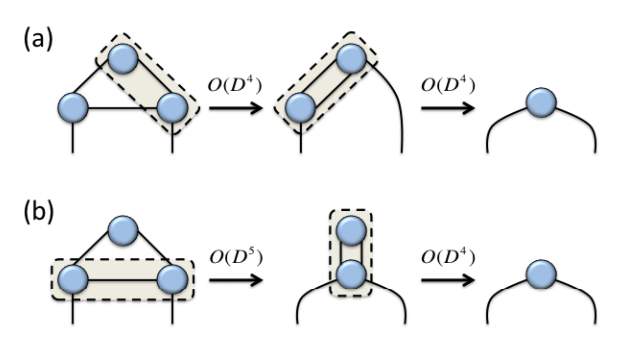
\includegraphics[width=0.8 \textwidth]{Figuren/tnalgs/contraction_order.png}
    \caption{ (a) Contraction of 3 tensors in $O(D^4)$ time (b) Contraction of same tensors in $O(D^5)$ time. Figure taken from \cite{Orus2014}.  }
    \label{fig:tnalgs:cont_ord}
\end{figure}